\documentclass[11pt,a4paper]{article}

\usepackage[utf8]{inputenc}
\usepackage[T1]{fontenc}
\usepackage{lmodern}
\usepackage[left=1.7cm,right=1.7cm,top=1.6cm,bottom=1.6cm]{geometry}
\usepackage{amsmath,amssymb}
\usepackage{booktabs,tabularx,array}
\usepackage{float}
\usepackage{tikz}
\usetikzlibrary{positioning,arrows.meta}
\usepackage{listings}
\usepackage{xcolor}
\usepackage[most]{tcolorbox}
\usepackage{hyperref}
\usepackage{enumitem}
\usepackage{caption}
\usepackage{titlesec}

\hypersetup{colorlinks=true,linkcolor=black,urlcolor=blue,citecolor=black}
\setlist{itemsep=2pt,topsep=3pt}
\setlength{\parindent}{0pt}
\setlength{\parskip}{5pt}
\titleformat{\section}{\Large\bfseries}{\thesection}{0.6em}{}
\titleformat{\subsection}{\large\bfseries}{\thesubsection}{0.6em}{}

\lstdefinelanguage{json}{
  basicstyle=\ttfamily\scriptsize,
  numbers=left,
  numberstyle=\tiny,
  stepnumber=1,
  numbersep=7pt,
  showstringspaces=false,
  breaklines=true,
  frame=single,
  columns=fullflexible
}
\lstset{breaklines=true,breakatwhitespace=false,columns=fullflexible}

\begin{document}

\begin{titlepage}
\centering
\vspace*{1.2cm}
{\Huge\bfseries DRIVE-TEST QoE RCA\par}
\vspace{0.5cm}
\begin{tcolorbox}[width=0.9\textwidth,colback=gray!5,colframe=gray!50]

\textbf{Focus:} Anomaly Monitoring, Repeated-Pattern Analysis, KPI-Based Root-Cause Reasoning, RCA Knowledge-Base Design, Deterministic Cause Matching, Evidence Extraction, Remediation Mapping, and LLM-Assisted Diagnostic Narration.
\end{tcolorbox}
\vfill
{\large August 2026\par}
\end{titlepage}

\tableofcontents
\newpage

\section{Executive Summary and System Architecture}

This report details the reasoning and explanation layer developed by Eman Tarek for the Drive-Test QoE Anomaly Detection \& Root Cause Analysis (RCA) system. While upstream modules convert raw, second-by-second LTE drive-test observations into statistical and machine-learning anomaly candidates, this contribution provides the engineering intelligence that transforms detected anomalies into actionable, explainable, and auditable network diagnoses.

The core design philosophy rests on two strict operational principles:

\begin{enumerate}
\item \textbf{KPI as Evidence, Not Cause:} Low RSRP or high Resource Block (RB) utilization are physical measurements, not root causes. The system maps measured evidence to explicit physical mechanisms such as \textit{Weak Serving Cell} or \textit{Cell Congestion}.

\item \textbf{Deterministic Rules Over Generative Hallucination:} The root-cause decision is made by a priority-ordered, deterministic rule engine grounded in 3GPP standards and telecom domain knowledge. The Large Language Model (LLM) is positioned strictly downstream as a diagnostic narrative layer to explain the structured verdict---it never independently invents or overrides a root cause.
\end{enumerate}

\begin{figure}[H]
\centering
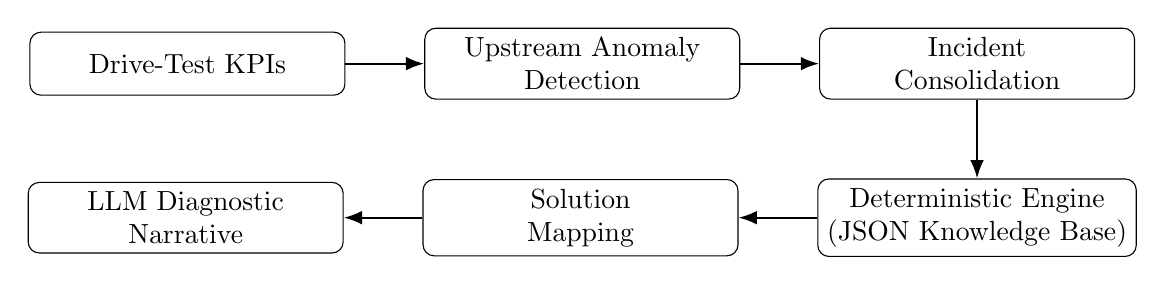
\begin{tikzpicture}[
box/.style={rectangle,rounded corners,draw,align=center,minimum width=4.0cm,minimum height=0.8cm},
arrow/.style={-{Latex},thick}
]
\node[box] (kpi) {Drive-Test KPIs};
\node[box,right=1.0cm of kpi] (anom) {Upstream Anomaly\\Detection};
\node[box,right=1.0cm of anom] (inc) {Incident\\Consolidation};
\node[box,below=1.0cm of inc] (eng) {Deterministic Engine\\(JSON Knowledge Base)};
\node[box,left=1.0cm of eng] (sol) {Solution\\Mapping};
\node[box,left=1.0cm of sol] (llm) {LLM Diagnostic\\Narrative};
\draw[arrow] (kpi)--(anom);
\draw[arrow] (anom)--(inc);
\draw[arrow] (inc)--(eng);
\draw[arrow] (eng)--(sol);
\draw[arrow] (sol)--(llm);
\end{tikzpicture}
\caption{Overall RCA and diagnostic architecture.}
\label{fig:architecture}
\end{figure}

\subsection{Scope and Population Metadata}

\begin{table}[H]
\centering
\small
\begin{tabularx}{\textwidth}{>{\bfseries}p{4.0cm} p{3.2cm} X}
\toprule
Metric / Parameter & Value & Description\\
\midrule
Primary Problem Scope & LTE DL Throughput Degradation & Focus on QoE degradation\\
Analysis Unit & Incident-Level Aggregate & Aggregated anomaly episodes with median KPI state\\
Total Incident Population & 1,382 & Analyzed incident cases\\
Underlying Drive-Test Rows & 2,824 & Raw observation samples represented\\
Unique Serving Cells (ECIs) & 423 & Distinct eNodeB sectors monitored\\
Unique Test Sessions & 254 & Distinct drive-test runs\\
Observation Window & Aug. 26, 2025 (23:37) $\rightarrow$ Aug. 29, 2025 (00:36) & Approximately 3-day monitoring period\\
Decision Layer & Deterministic, Priority-Ordered, KPI-Driven & Knowledge base via \texttt{causes.json} and \texttt{kpi\_rules.json}\\
Explanation Layer & LLM-Assisted Narrative Generation & Converts structured JSON verdict into engineer reports\\
\bottomrule
\end{tabularx}
\caption{Scope and population metadata.}
\end{table}

\section{Contributor Responsibilities and Boundary Definition}

Within the project work plan, Eman Tarek owns the complete pipeline between upstream anomaly detection handoff and final downstream diagnostic representation.

\begin{table}[H]
\centering
\small
\begin{tabularx}{\textwidth}{>{\bfseries}p{3.4cm} p{6.0cm} X}
\toprule
Functional Module & Technical Responsibility & Primary Technical Output\\
\midrule
Anomaly Monitoring & Consolidates raw anomaly rows into persistent, repeated incident cases. & Prioritized Incident Cases\\
RCA Cause Taxonomy & Defines the hierarchical priority structure of engineering causes. & Priority Cause Tree\\
Knowledge Base Architecture & Designs the decoupled three-JSON system (\texttt{causes}, \texttt{kpi\_rules}, \texttt{solutions}). & Maintainable Knowledge Base\\
KPI Reasoning Engine & Implements rule evaluation logic (\texttt{MATCH\_ALL}/\texttt{MATCH\_ANY}) against evidence. & Primary Cause ID + Evidence Trace\\
Evidence Extraction & Extracts and formats exact KPI values supporting the selected cause. & \texttt{key\_kpi\_evidence} Payload\\
Remediation Mapping & Links confirmed cause IDs to standardized telecom remediation actions. & \texttt{recommended\_solution} Entry\\
LLM Diagnostic Layer & Prompts LLM to render structured RCA JSON into natural diagnostic prose. & Human-Readable Diagnostic Narrative\\
\bottomrule
\end{tabularx}
\caption{Contributor responsibilities and technical outputs.}
\end{table}

\textbf{Scope Boundary:} Upstream anomaly detection (flagging a drop) is treated as an input. This contribution explains \textit{why} the degradation occurred, \textit{how confident} the system is, and \textit{what actions} engineers should take. Planning data is treated as an independent stream and is never used as proof for drive-test anomalies due to spatial mismatches.

\section{Data and KPI Taxonomy}

The RCA engine evaluates multi-dimensional drive-test telemetry grouped into distinct functional groups.

\begin{table}[H]
\centering
\scriptsize
\begin{tabularx}{\textwidth}{>{\bfseries}p{3.0cm} p{5.0cm} X}
\toprule
KPI Group & Specific Metrics / Indicators & Engineering Significance in RCA\\
\midrule
Throughput (Symptom) & Actual DL Throughput, Expected $p_{75}$ Throughput, Throughput Gap & Defines performance drop severity and baseline gap\\
Coverage & RSRP (Serving Cell) & Identifies weak coverage and cell-edge conditions\\
Radio Quality & RSRQ, SINR & Separates inter-cell interference from signal attenuation\\
Link Adaptation & CQI, MCS, BLER & Evaluates channel state reporting and modulation efficiency\\
Resource Allocation & RB Utilization, Cell PRB Load, Throughput/RB & Detects air-interface congestion versus scheduler under-grant\\
Carrier Aggregation (CA) & CA Active Flag, Carrier Count, SCell1 RSRP/SINR/CQI/BLER & Identifies secondary carrier underperformance or deactivation\\
Mobility & HO Count ($\pm5$ s), Dwell Time, Serving-Neighbor RSRP Delta, UE Speed & Evaluates handover timing, ping-ponging, and neighbor relations\\
Access & RACH Failure Flag, RACH Attempts, Access Delay & Identifies random-access channel contention and link setup failures\\
MIMO / Spatial & Rank Indicator (RI), Layer Utilization & Detects rank fallback (RI=1) under strong SINR conditions\\
\bottomrule
\end{tabularx}
\caption{KPI taxonomy used by the RCA engine.}
\end{table}

\section{RCA Reasoning Framework and Taxonomy}

To prevent a single degraded KPI, such as high BLER, from falsely triggering a diagnosis, the framework enforces a \textbf{priority-ordered evaluation hierarchy}. Causes higher in the hierarchy are evaluated first; if their defining gate conditions are met, the evaluation halts, ensuring traceable and deterministic decision-making.

\begin{figure}[H]
\centering
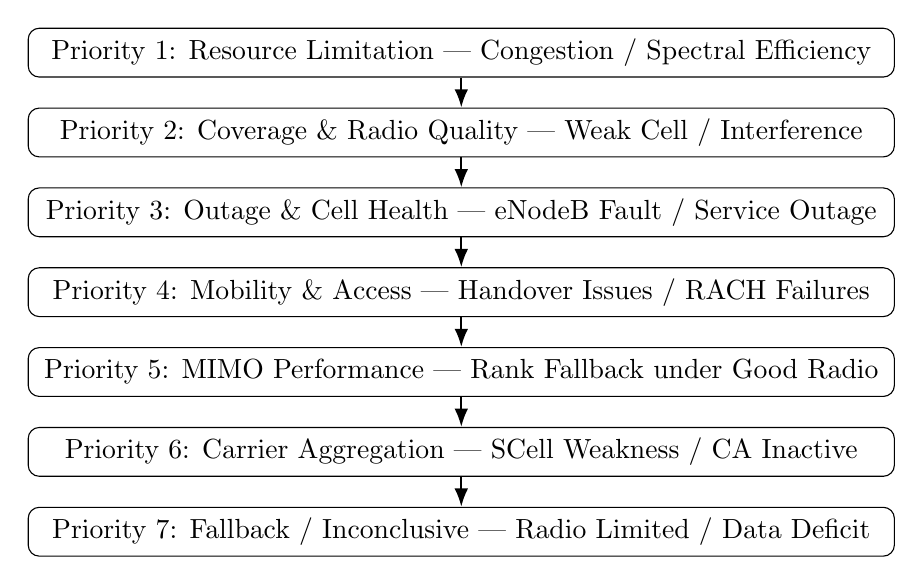
\begin{tikzpicture}[node distance=0.38cm,
box/.style={rectangle,rounded corners,draw,align=center,minimum width=11cm,minimum height=0.62cm},
arrow/.style={-{Latex},thick}]
\node[box] (p1) {Priority 1: Resource Limitation --- Congestion / Spectral Efficiency};
\node[box,below=of p1] (p2) {Priority 2: Coverage \& Radio Quality --- Weak Cell / Interference};
\node[box,below=of p2] (p3) {Priority 3: Outage \& Cell Health --- eNodeB Fault / Service Outage};
\node[box,below=of p3] (p4) {Priority 4: Mobility \& Access --- Handover Issues / RACH Failures};
\node[box,below=of p4] (p5) {Priority 5: MIMO Performance --- Rank Fallback under Good Radio};
\node[box,below=of p5] (p6) {Priority 6: Carrier Aggregation --- SCell Weakness / CA Inactive};
\node[box,below=of p6] (p7) {Priority 7: Fallback / Inconclusive --- Radio Limited / Data Deficit};
\draw[arrow](p1)--(p2); \draw[arrow](p2)--(p3); \draw[arrow](p3)--(p4);
\draw[arrow](p4)--(p5); \draw[arrow](p5)--(p6); \draw[arrow](p6)--(p7);
\end{tikzpicture}
\caption{Priority-ordered RCA hierarchy.}
\end{figure}

\subsection{Priority 1: Resource Limitation}

\textbf{Cell Congestion (C01):} Triggered when user demand is confirmed, RB usage is saturated ($\ge80\%$), and actual throughput falls significantly below expected baselines ($<75\%$).

\textbf{Poor Spectral Efficiency (C02):} Triggered when demand exists and RB allocation is low ($<40\%$), but throughput per RB is degraded while radio quality remains acceptable.

\subsection{Priority 2: Coverage and Radio Quality}

\textbf{Weak Serving Cell (C03):} Requires \texttt{MATCH\_ALL} logic across signal parameters:
\[
RSRP<-105\,\mathrm{dBm},\quad RSRQ<-15\,\mathrm{dB},\quad MCS<10,\quad BLER>10\%.
\]

\textbf{Radio Link Failure / Interference (C04):} Requires acceptable coverage ($RSRP\ge-105$ dBm) combined with poor quality ($SINR<0$ dB or $RSRQ<-15$ dB) and high BLER ($>10\%$).

\subsection{Priority 3: Outage and Cell Health}

\textbf{Serving Cell / eNodeB Fault (C05):} Identified by near-zero throughput ($<0.05$ Mbps) or joint KPI collapse while UE radio metrics remain normal, ruling out coverage/interference.

\textbf{Neighbor Cell Outage (C06):} Identified when local serving KPIs are normal ($RSRP\ge-105$ dBm, $SINR\ge0$ dB), but local RB utilization spikes sharply as the cell absorbs redirected traffic from a failed neighbor.

\subsection{Priority 4: Mobility and Access}

\textbf{Handover Problem (C07):} Evaluates late handovers ($Serving-Neighbor~RSRP<-6$ dB), ping-pong handovers (dwell $<5$ s or HO count $\ge95$th percentile), and high-speed degradation ($\ge60$ km/h).

\textbf{Access Failures (C08):} Triggered by repeated RACH attempts ($\ge3$), high access latency, or elevated RACH failure rates ($>5\%$).

\subsection{Priority 5: MIMO Performance}

\textbf{Poor Spatial Multiplexing (C09):} Triggered when $SINR\ge20$ dB but $RI=1$, pointing to antenna correlation, feeder cable faults, or PIM issues.

\subsection{Priority 6: Carrier Aggregation}

\textbf{Weak Secondary Cell (C10):} Active CA ($carrier\_count\ge2$), but SCell1 shows $RSRP<-105$ dBm and $SINR<0$ dB.

\textbf{SCell Release / Deactivation (C11):} Secondary carrier drops mid-episode following high SCell BLER ($>10\%$).

\textbf{CA Inactive / Disabled (C12):} Primary carrier operates alone ($carrier\_count=1$) despite potential CA capability.

\subsection{Priority 7: Fallback / Inconclusive}

\textbf{Radio Limited (C13):} Unclassified moderate link degradation ($BLER>10\%$ or $CQI\le7$) without matching higher-priority gates.

\textbf{Inconclusive (C14):} Unconfirmed user demand or insufficient evidence to assign a specific engineering cause.

\section{Knowledge Base Architecture: The Three-JSON System}

To prevent domain knowledge from being hardcoded inside Python scripts, the RCA architecture separates concerns across three JSON files linked by stable identifiers (\texttt{Cause ID} and \texttt{Solution ID}).

\begin{figure}[H]
\centering
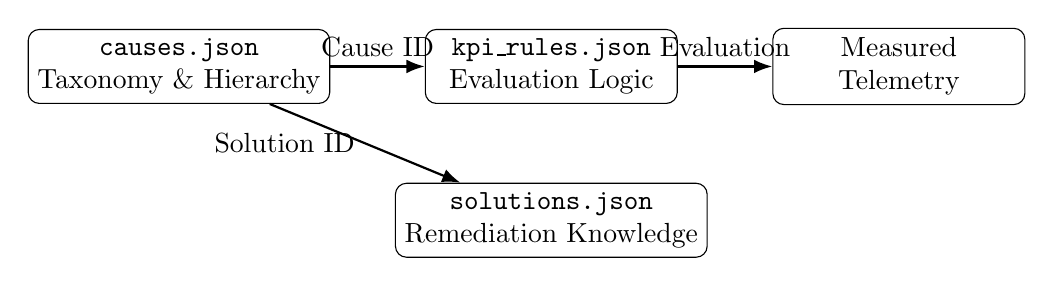
\begin{tikzpicture}[node distance=1.0cm and 1.2cm,
box/.style={rectangle,rounded corners,draw,align=center,minimum width=3.2cm,minimum height=0.9cm},
arrow/.style={-{Latex},thick}]
\node[box](c){\texttt{causes.json}\\Taxonomy \& Hierarchy};
\node[box,right=of c](r){\texttt{kpi\_rules.json}\\Evaluation Logic};
\node[box,right=of r](t){Measured\\Telemetry};
\node[box,below=of r](s){\texttt{solutions.json}\\Remediation Knowledge};
\draw[arrow](c)--node[above]{Cause ID}(r);
\draw[arrow](r)--node[above]{Evaluation}(t);
\draw[arrow](c)--node[left]{Solution ID}(s);
\end{tikzpicture}
\caption{Three-JSON knowledge-base architecture.}
\end{figure}

\begin{table}[H]
\centering
\small
\begin{tabularx}{\textwidth}{>{\ttfamily}p{3.0cm} >{\bfseries}p{4.0cm} X}
\toprule
JSON File & Core System Role & Key Content and Schema\\
\midrule
causes.json & Taxonomy \& Hierarchy & Priority levels, category definitions, subcause lists, cause IDs (C01--C14), solution IDs (SOL\_C01), and string templates (\texttt{reason\_template}).\\
kpi\_rules.json & Evaluation Logic \& Thresholds & Exact KPI JSON paths, comparison operators, numerical thresholds, evaluation modes (\texttt{MATCH\_ALL} vs. \texttt{MATCH\_ANY}), and gate conditions.\\
solutions.json & Remediation Knowledge & Solution IDs, recommended engineering actions, investigation steps, 3GPP specification standards, and vendor documentation references.\\
\bottomrule
\end{tabularx}
\caption{Knowledge-base component summary.}
\end{table}

\section{Deterministic RCA Engine Execution Flow}

The classification script (\texttt{classify\_incidents.py}) executes a rule-driven pipeline at runtime:

\begin{enumerate}
\item \textbf{Load Artifacts:} Parses \texttt{causes.json}, \texttt{kpi\_rules.json}, \texttt{solutions.json}, and input incident records.
\item \textbf{Extract Telemetry:} Extracts raw and derived KPI fields using a safe extractor (\texttt{extract\_fields()}).
\item \textbf{Evaluate Hierarchy:} Sequentially tests cause gates from Priority 1 to Priority 7.
\item \textbf{Apply Boolean Logic:} Evaluates \texttt{MATCH\_ALL} or \texttt{MATCH\_ANY} conditions. If a gate fires, evaluation halts.
\item \textbf{Format Reason Template:} Populates the cause's \texttt{reason\_template} with actual KPI values rounded to two decimal places.
\item \textbf{Attach Solution:} Fetches corresponding actions and standards citations from \texttt{solutions.json}.
\item \textbf{Emit Structured Output:} Writes the final JSON payload.
\end{enumerate}

\subsection{Standardized RCA Output Schema Example}

\begin{lstlisting}[language=json,caption={Example standardized RCA output.}]
{
  "incident_id": "INC-2025-08-28-1066034",
  "diagnosis": {
    "category": "Resource Limitation",
    "cause_name": "PRB Allocation / Capacity-Limited",
    "cause_id": "C01",
    "severity": "High",
    "reason": "This anomaly is capacity-limited: the UE had confirmed download demand, was using 96.0% of available RB capacity across 1.0 carrier(s), falling 13.68 Mbps below expected throughput."
  },
  "key_kpi_evidence": {
    "actual_throughput_mbps": 0.03,
    "expected_throughput_mbps": 0.47,
    "rsrp_dbm": -104.58,
    "sinr_db": 8.44,
    "cqi": 8.0,
    "mcs": 10.0,
    "bler_pct": 11.76,
    "rb_usage_pct": 96.0
  },
  "evaluation_trace": {
    "priority_1_to_4": {
      "C01": {
        "matched": true,
        "sub_evidence": {
          "C01_a": true,
          "C01_b": "NOT_COMPUTABLE",
          "C01_e": false
        }
      }
    }
  },
  "recommended_solution": {
    "solution_id": "SOL_C01",
    "recommended_actions": [
      "Check cell-level PRB utilization counters in OSS to confirm macro-level sector congestion.",
      "Evaluate carrier aggregation configuration and secondary carrier availability to offload traffic.",
      "Consider physical layer expansion or active load-balancing parameter tuning."
    ],
    "standards_and_vendor_references": [
      {
        "source": "3GPP TS 36.331 / Vendor PRB Optimization Guide",
        "note": "PRB utilization exceeding 80% represents severe air-interface saturation."
      }
    ]
  }
}
\end{lstlisting}

\section{Incident-Level Empirical Results (1,382 Incidents)}

The RCA engine was executed against the dataset of 1,382 incident-level aggregates.

\subsection{Root-Cause Distribution Summary}

\begin{table}[H]
\centering
\tiny
\begin{tabularx}{\textwidth}{c X r r X}
\toprule
Cause ID & Engineering Cause Name & Count & Share & Dominant Category\\
\midrule
C01 & Cell Congestion (Capacity-Limited) & 365 & 26.4\% & Resource Limitation\\
C03 & Weak Serving Cell & 237 & 17.1\% & Coverage \& Radio Quality\\
C14 & Inconclusive (Insufficient Evidence) & 236 & 17.1\% & Fallback\\
C13 & Radio Limited (Link Adaptation) & 181 & 13.1\% & Fallback\\
C06 & Neighbor Cell Outage / Load Shift & 98 & 7.1\% & Outage \& Cell Health\\
C12 & CA Inactive / Disabled & 92 & 6.7\% & Carrier Aggregation\\
C10 & Weak Secondary Cell (SCell) & 40 & 2.9\% & Carrier Aggregation\\
C07\_a & Handover Problem -- Late Handover & 35 & 2.5\% & Mobility \& Access\\
C09 & MIMO Rank Fallback & 33 & 2.4\% & MIMO\\
C04 & Interference / Radio Link Failure & 28 & 2.0\% & Coverage \& Radio Quality\\
C08 & Access Problem (RACH Failures) & 18 & 1.3\% & Mobility \& Access\\
C07\_c & Handover Problem -- Ping-Pong HO & 9 & 0.7\% & Mobility \& Access\\
C05 & Serving Cell / eNodeB Fault & 5 & 0.4\% & Outage \& Cell Health\\
C02 & Poor Spectral Efficiency & 5 & 0.4\% & Resource Limitation\\
\midrule
\textbf{Total} & \textbf{All Categories} & \textbf{1,382} & \textbf{100.0\%} &\\
\bottomrule
\end{tabularx}
\caption{Root-cause distribution across 1,382 incidents.}
\end{table}

\subsection{Key Engineering Findings}

\begin{enumerate}
\item \textbf{Resource Saturation Dominance:} Cell Congestion (C01) represents the single largest cause (26.4\%, 365 incidents). These cases occurred under verified download demand where RBs were saturated, indicating that capacity expansion or traffic offloading is required rather than RF tuning.

\item \textbf{Coverage Limits:} Weak Serving Cell (C03) represents 17.1\% (237 incidents), confirming that RF attenuation remains a major bottleneck in the drive-test area.

\item \textbf{Operational Trust via Inconclusive Classification:} Inconclusive (C14) accounts for 17.1\% (236 incidents). This is a critical feature of the system: when drive-test data lacks necessary fields, such as missing OSS alarms or unconfirmed demand, the engine defaults to Inconclusive rather than generating false diagnoses.
\end{enumerate}

\section{Remediation Mapping Engine}

Once a root cause is established, the engine retrieves corresponding remediation guidelines from \texttt{solutions.json}.

\begin{table}[H]
\centering
\scriptsize
\begin{tabularx}{\textwidth}{>{\bfseries}p{3.0cm} p{4.0cm} X}
\toprule
Cause Category & Primary Engineering Root Cause & Direct Remediation Action\\
\midrule
Resource Limitation & Cell Congestion (C01) & Trigger carrier expansion, adjust inter-frequency load balancing (IFLB), optimize PRB scheduling, or deploy small cells.\\
Coverage \& Radio & Weak Serving Cell (C03) & Audit antenna downtilt/azimuth, increase RS transmission power, or evaluate site placement/coverage expansion.\\
Coverage \& Radio & Interference (C04) & Audit frequency planning, adjust antenna tilts to reduce overshoot, investigate external interference, or tune PCI/PDSCH power offsets.\\
Outage \& Health & Serving Cell Fault (C05) & Inspect OSS alarm logs for eNodeB board failures, transmission backhaul drops, or power amplifier limits before dispatching RF teams.\\
Mobility & Late Handover (C07\_a) & Decrease Event A3 offset/hysteresis, reduce Time-to-Trigger (TTT), or audit Neighbor Relation Tables (NRT).\\
Mobility & Ping-Pong Handover (C07\_c) & Increase Event A3 hysteresis margin, adjust Cell Individual Offsets (CIO), or increase hysteresis timers.\\
MIMO & Rank Fallback (C09) & Inspect physical antenna paths, feeder cables, VSWR ratios, and PIM levels; check UE transmission mode (TM) configuration.\\
Carrier Aggregation & Weak Secondary Cell (C10) & Audit SCell coverage/tilt, adjust A5/A2 thresholds for SCell addition/release, or re-evaluate SCell frequency band choice.\\
\bottomrule
\end{tabularx}
\caption{Cause-to-remediation mapping.}
\end{table}

\section{Downstream LLM Diagnostic Narration}

The Large Language Model (LLM) operates strictly as a text-generation layer downstream of the deterministic RCA engine. It translates structured JSON verdicts into concise diagnostic reports for Network Operations Center (NOC) engineers.

\subsection{Recommended Prompting Structure}

\begin{enumerate}
\item \textbf{Context \& Symptom:} State the incident ID, timestamp, serving cell, and throughput drop.
\item \textbf{Deterministic Verdict:} State the primary cause name and cause ID (C01--C14).
\item \textbf{KPI Evidence:} Cite the exact numerical KPI values that triggered the decision rule.
\item \textbf{Reasoning Explanation:} Explain why the KPI combination supports this physical mechanism.
\item \textbf{Action Plan:} Present the recommended remediation steps from \texttt{solutions.json}.
\end{enumerate}

\begin{tcolorbox}[title=System Guardrail,colback=gray!5,colframe=black!60]
The LLM prompt strictly instructs the model to explain the deterministic verdict. It is forbidden from altering the assigned \texttt{cause\_id}, inventing unmeasured KPIs, or proposing remedies outside \texttt{solutions.json}.
\end{tcolorbox}

\section{System Validation and Explainability Audit}

The system's architecture directly addresses key engineering auditability requirements.

\begin{table}[H]
\centering
\small
\begin{tabularx}{\textwidth}{>{\bfseries}p{5.0cm} X}
\toprule
Engineering Question & System Audit Mechanism\\
\midrule
Why was this cause selected? & Traced to a specific priority rule gate in \texttt{kpi\_rules.json} that was satisfied.\\
Which KPIs support the decision? & All matching KPI values are explicitly stored in the \texttt{key\_kpi\_evidence} JSON payload.\\
Can thresholds be updated? & Yes. Modifying values in \texttt{kpi\_rules.json} changes behavior without editing Python code.\\
Can remedies be customized? & Yes. Updating \texttt{solutions.json} updates engineering recommendations system-wide.\\
How are data gaps handled? & Missing fields are flagged as \texttt{NOT\_COMPUTABLE}, preventing false conclusions.\\
Can an engineer override the output? & Yes. The structured JSON retains full evaluation traces (\texttt{evaluation\_trace}) for manual review.\\
Does the LLM introduce hallucinated causes? & No. The cause decision is finalized before the LLM prompt is constructed.\\
\bottomrule
\end{tabularx}
\caption{Explainability and auditability mechanisms.}
\end{table}

\section{Future Work and Enhancements}

\begin{enumerate}
\item \textbf{Row-Level Sequential RCA:} Extend the engine from incident-level aggregates to row-level time-series data to capture real-time state transitions, such as mid-session SCell drops.

\item \textbf{OSS \& Alarm Integration:} Ingest eNodeB hardware alarms, MME paging logs, and backhaul status counters to resolve C05/C06 outage sub-causes.

\item \textbf{Dynamic Cell-Specific Baselines:} Replace static global thresholds ($RSRP<-105$ dBm) with cell-specific historical percentiles ($p_{10}/p_{50}$).

\item \textbf{Enhanced Evidence Scoring:} Implement a multi-factor confidence score based on the number and independence of supporting KPI indicators.

\item \textbf{LLM Verification Guard:} Implement an automated validation check that compares generated text against the source JSON to ensure 100\% factual alignment.
\end{enumerate}

\section{Conclusion}

This contribution establishes an auditable, rule-driven Root Cause Analysis framework for LTE drive-test throughput anomalies. By enforcing a deterministic decision layer backed by a modular three-JSON knowledge base, the system converts raw telemetry into clear engineering diagnoses linked to actionable remediation steps.

Applied to the 1,382-incident evaluation dataset, the engine identified \textbf{Cell Congestion} (26.4\%) and \textbf{Weak Serving Cell} (17.1\%) as the primary network bottlenecks, while maintaining operational trust by categorizing ambiguous cases as \textbf{Inconclusive} (17.1\%).

The downstream LLM layer converts these structured verdicts into clear diagnostic prose without sacrificing deterministic rigor.

\begin{tcolorbox}[title=Technical Pipeline Summary,colback=gray!5,colframe=black!60]
\centering
\texttt{Detected Anomaly}
$\rightarrow$
\texttt{Monitored Incident}
$\rightarrow$
\texttt{KPI Evidence Extraction}
$\rightarrow$
\texttt{Deterministic Rule Match}
$\rightarrow$
\texttt{Remediation Retrieval}
$\rightarrow$
\texttt{LLM Diagnostic Narrative}
\end{tcolorbox}

\appendix
\section{Suggested Schema for Downstream Integration}

\begin{table}[H]
\centering
\small
\begin{tabularx}{\textwidth}{>{\ttfamily}p{4.0cm} >{\ttfamily}p{3.0cm} X}
\toprule
Field Name & Data Type & Purpose\\
\midrule
incident\_id & String & Unique source incident identifier\\
timestamp & ISO-8601 String & Incident start/end window\\
serving\_cell\_eci & Float/String & E-UTRAN Cell Identifier (ECI)\\
primary\_cause\_id & String & Stable cause identifier (e.g., C01, C03)\\
primary\_cause\_name & String & Human-readable engineering cause name\\
severity & String & Incident severity level (Critical, High, Medium)\\
reason\_statement & String & Formatted, evidence-populated explanation string\\
key\_kpi\_evidence & JSON Object & Dictionary of measured KPI values used in rule matching\\
evaluation\_trace & JSON Object & Complete audit trail of evaluated priority gates\\
recommended\_actions & Array of Strings & Specific engineering steps retrieved from \texttt{solutions.json}\\
standards\_references & Array of Objects & 3GPP and vendor documentation citations\\
\bottomrule
\end{tabularx}
\caption{Suggested downstream integration schema.}
\end{table}

\end{document}
